\documentclass{standalone}

\usepackage{tikz}
\usepackage{circuitikz}

\tikzset{block/.style = {draw, fill=white, very thick, rectangle, minimum height=1cm, minimum width=2cm},
         lblock/.style={draw,fill=white,very thick, rectangle, minimum height=3cm, minimum width=1cm},
         sum/.style= {draw, fill=white, very thick, circle, node distance=0.5cm}}

         
\begin{document}
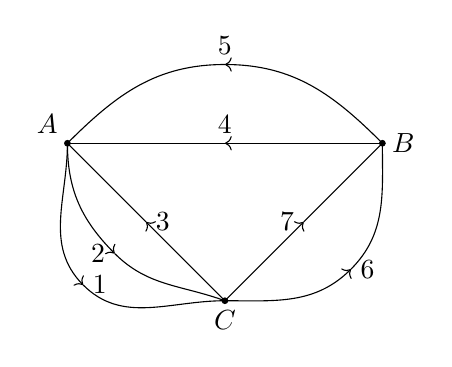
\begin{tikzpicture}[scale=2]
    \filldraw[black](0,0)circle(0.5pt);
    \filldraw[black](2,0)circle(0.5pt);
    \filldraw[black](1,-1)circle(0.5pt);

    \draw[->](2,0)--(1,0)node[above]{$4$};
    \draw[-](1,0)--(0,0)node[above left]{$A$};

    \draw[->](1,-1)--(0.5,-0.5)node[right]{$3$};
    \draw[-](0.5,-0.5)--(0,0);

    \draw[->](1,-1)node[below]{$C$}--(1.5,-0.5)node[left]{$7$};
    \draw[-](1.5,-0.5)--(2,0)node[right]{$B$};

    \draw[->](2,0)to[out=135,in=0](1,0.5)node[above]{$5$};
    \draw[-](1,0.5)to[out=180,in=45](0,0);

    \draw[->](1,-1)to[out=0,in=225](1.8,-0.8)node[right]{$6$};
    \draw[-](1.8,-0.8)to[out=45,in=270](2,0);

    \draw[-](1,-1)to[out=160,in=315](0.3,-0.7)node[left]{$2$};
    \draw[<-](0.3,-0.7)to[out=135,in=270](0,0);

    \draw[-](1,-1)to[out=180,in=315](0.1,-0.9)node[right]{$1$};
    \draw[<-](0.1,-0.9)to[out=135,in=270](0,0);
\end{tikzpicture}
\end{document}